\section{GPIO \refskript{8.1, 8.2}}
\begin{lstlisting}[language=C++]
PxDIR &= ~0x01;	// Set Px.0 as input
PxDIR |=  0x02;	// Set Px.1 as output
PxOUT &= ~0x02;	// Clear LED on Px.1

...
while(1) {
	while (PxIN & 0x01) {} // wait for SW1 pressed
	PxOUT ^=  0x02; // toggle LED D1 on Px.1
	while (!(PxIN & 0x01)) {} // wait for SW1 pressed
}
\end{lstlisting}\vspace{-25px}
\begin{lstlisting}[language=C++]
PxDIR &= ~0x01;	// Set Px.0 as input
PxOUT |=  0x01;	// Use pullup resistor on Px.0
PxREN |=  0x01; // Enable pullup resistor on Px.0
\end{lstlisting}\vspace{-20px}

Voltage divider for down-conversion.
\begin{center}
	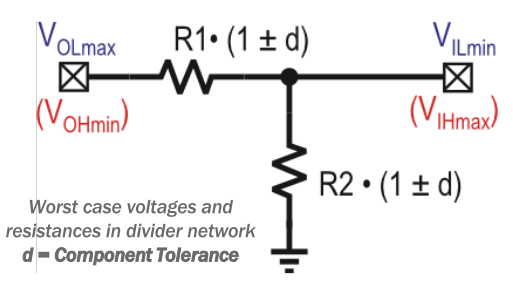
\includegraphics[width=.6\columnwidth]{"Images/Voltage_Divider.png"}
\end{center}






